\begin{figure}[H]
    \centering
    



\tikzset{every picture/.style={line width=0.75pt}} %set default line width to 0.75pt        

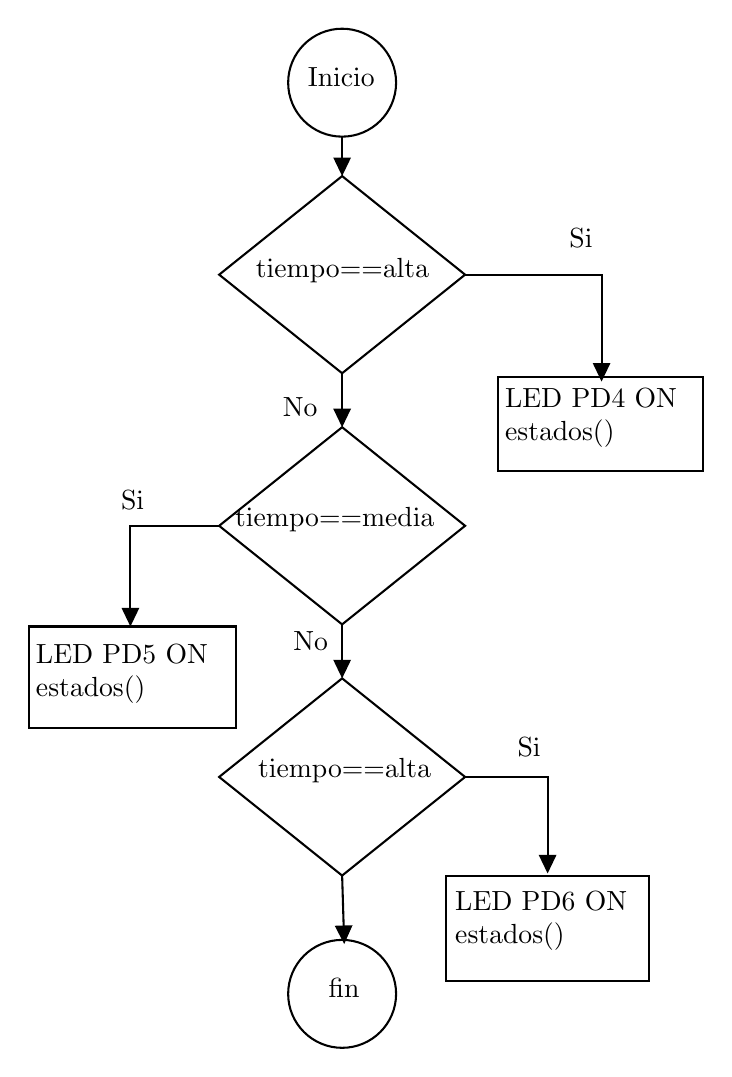
\begin{tikzpicture}[x=0.75pt,y=0.75pt,yscale=-1,xscale=1]
%uncomment if require: \path (0,606); %set diagram left start at 0, and has height of 606

%Flowchart: Connector [id:dp021633046726569516] 
\draw   (290,58) .. controls (290,43.64) and (301.64,32) .. (316,32) .. controls (330.36,32) and (342,43.64) .. (342,58) .. controls (342,72.36) and (330.36,84) .. (316,84) .. controls (301.64,84) and (290,72.36) .. (290,58) -- cycle ;
%Flowchart: Decision [id:dp3699261934488949] 
\draw   (316,103) -- (375.25,150.5) -- (316,198) -- (256.75,150.5) -- cycle ;
%Straight Lines [id:da9331918609664245] 
\draw    (316,84) -- (316,100) ;
\draw [shift={(316,103)}, rotate = 270] [fill={rgb, 255:red, 0; green, 0; blue, 0 }  ][line width=0.08]  [draw opacity=0] (8.93,-4.29) -- (0,0) -- (8.93,4.29) -- cycle    ;
%Shape: Right Angle [id:dp2526929905854485] 
\draw   (375.25,150.5) -- (441,150.5) -- (441,176) ;
%Straight Lines [id:da07125413731798624] 
\draw    (441,176) -- (441,199) ;
\draw [shift={(441,202)}, rotate = 270] [fill={rgb, 255:red, 0; green, 0; blue, 0 }  ][line width=0.08]  [draw opacity=0] (8.93,-4.29) -- (0,0) -- (8.93,4.29) -- cycle    ;
%Flowchart: Process [id:dp7214387169012859] 
\draw   (391,200) -- (490,200) -- (490,245) -- (391,245) -- cycle ;
%Straight Lines [id:da2715179028720167] 
\draw    (316,198) -- (316,221) ;
\draw [shift={(316,224)}, rotate = 270] [fill={rgb, 255:red, 0; green, 0; blue, 0 }  ][line width=0.08]  [draw opacity=0] (8.93,-4.29) -- (0,0) -- (8.93,4.29) -- cycle    ;
%Flowchart: Process [id:dp9789563686318568] 
\draw   (366,440) -- (464,440) -- (464,491) -- (366,491) -- cycle ;
%Flowchart: Decision [id:dp1028100469525679] 
\draw   (316,224) -- (375.25,271.5) -- (316,319) -- (256.75,271.5) -- cycle ;
%Shape: Right Angle [id:dp7584861080562588] 
\draw   (256.75,271.5) -- (214,271.5) -- (214,294) ;
%Straight Lines [id:da2270209718957621] 
\draw    (415,413) -- (415,436) ;
\draw [shift={(415,439)}, rotate = 270] [fill={rgb, 255:red, 0; green, 0; blue, 0 }  ][line width=0.08]  [draw opacity=0] (8.93,-4.29) -- (0,0) -- (8.93,4.29) -- cycle    ;
%Straight Lines [id:da8351372179661163] 
\draw    (214,294) -- (214,317) ;
\draw [shift={(214,320)}, rotate = 270] [fill={rgb, 255:red, 0; green, 0; blue, 0 }  ][line width=0.08]  [draw opacity=0] (8.93,-4.29) -- (0,0) -- (8.93,4.29) -- cycle    ;
%Flowchart: Process [id:dp3175001957530377] 
\draw   (165,320) -- (265,320) -- (265,369) -- (165,369) -- cycle ;
%Straight Lines [id:da6198639865714966] 
\draw    (316,319) -- (316,342) ;
\draw [shift={(316,345)}, rotate = 270] [fill={rgb, 255:red, 0; green, 0; blue, 0 }  ][line width=0.08]  [draw opacity=0] (8.93,-4.29) -- (0,0) -- (8.93,4.29) -- cycle    ;
%Flowchart: Decision [id:dp2817555903877169] 
\draw   (316,345) -- (375.25,392.5) -- (316,440) -- (256.75,392.5) -- cycle ;
%Shape: Right Angle [id:dp6691165773669392] 
\draw   (375.25,392.5) -- (415,392.5) -- (415,413) ;
%Straight Lines [id:da7899754118364894] 
\draw    (316,440) -- (316.91,470) ;
\draw [shift={(317,473)}, rotate = 268.26] [fill={rgb, 255:red, 0; green, 0; blue, 0 }  ][line width=0.08]  [draw opacity=0] (8.93,-4.29) -- (0,0) -- (8.93,4.29) -- cycle    ;
%Flowchart: Connector [id:dp5690598454040376] 
\draw   (290,497) .. controls (290,482.64) and (301.64,471) .. (316,471) .. controls (330.36,471) and (342,482.64) .. (342,497) .. controls (342,511.36) and (330.36,523) .. (316,523) .. controls (301.64,523) and (290,511.36) .. (290,497) -- cycle ;

% Text Node
\draw (298,49) node [anchor=north west][inner sep=0.75pt]   [align=left] {Inicio};
% Text Node
\draw (273,141) node [anchor=north west][inner sep=0.75pt]   [align=left] {tiempo==alta};
% Text Node
\draw (263,261) node [anchor=north west][inner sep=0.75pt]   [align=left] {tiempo==media};
% Text Node
\draw (393,204) node [anchor=north west][inner sep=0.75pt]   [align=left] {LED PD4 ON\\estados()};
% Text Node
\draw (369,446) node [anchor=north west][inner sep=0.75pt]   [align=left] {LED PD6 ON\\estados()};
% Text Node
\draw (167,327) node [anchor=north west][inner sep=0.75pt]   [align=left] {LED PD5 ON\\estados()};
% Text Node
\draw (424,127) node [anchor=north west][inner sep=0.75pt]   [align=left] {Si};
% Text Node
\draw (286,208) node [anchor=north west][inner sep=0.75pt]   [align=left] {No};
% Text Node
\draw (291,321) node [anchor=north west][inner sep=0.75pt]   [align=left] {No};
% Text Node
\draw (274,382) node [anchor=north west][inner sep=0.75pt]   [align=left] {tiempo==alta};
% Text Node
\draw (399,372) node [anchor=north west][inner sep=0.75pt]   [align=left] {Si};
% Text Node
\draw (208,253) node [anchor=north west][inner sep=0.75pt]   [align=left] {Si};
% Text Node
\draw (308,488) node [anchor=north west][inner sep=0.75pt]   [align=left] {fin};


\end{tikzpicture}


\caption{Diagrama de flujo función led\_carga.}
\label{sch2}
\end{figure}